\documentclass[rascunho,xindy,table]{fei}
 \setlength{\footskip}{4.32004pt}

\PassOptionsToPackage{brazil,portuguese,english}{babel} 
\usepackage{babel} 
\usepackage[utf8]{inputenc}
\usepackage{longtable}
\usepackage{rotating}
\usepackage{xcolor,colortbl}
\usepackage{booktabs}
\usepackage{graphicx}
\usepackage{caption}
\usepackage{subcaption}
\usepackage{pdfpages}
\usepackage{enumitem}
\usepackage{float}
\usepackage{graphicx}
\usepackage{graphics}

\usepackage{hyperref}
\hypersetup{
    colorlinks=true,
    linkcolor=blue,
    filecolor=magenta,      
    urlcolor=blue,
    pdfpagemode=FullScreen,
    }

\author{
    Bruno Orlandin R.A.: 22.219.032-4\\
    Shawn Kawabe R.A.: 22.219.013-4\\
}
\title{Atividade 2: Função Hash}

%\cidade{Cidade}
\instituicao{CENTRO UNIVERSITÁRIO FEI}

\newacronym[longplural=Centro Universitário FEI]{fei}{FEI}{Centro Universitário FEI}

\begin{document}

\maketitle

\href{https://github.com/shawnkawabe/hash-fei.git}{Repositório do Github com o código fonte}

\chapter{Introducao} \label{intro}

Está atividade consiste verificar a autenticidade por meio de Hashes, que serão 
gerados do cálculo das funnções SHA-256 e MD5. Cada frase contém seus Hashes ao lado
e para verificar a autenticidade das frases, serão gerados os Hashes de cadas e 
caso os mesmos sejam iguais aos dados, a frase é verdadeira.
\chapter{Código} \label{codigo}

Para a codificação dessa atividade foi utilizada a linguagem de programação Python.
A geração dos Hashes das frases foi feita utilizando a bilbioteca hashlib. Para 
tornar o programa mais dinâmico, as frases e os Hashes que foram analisados foram 
colocados em um arquivo texto (list.txt) para que fosse possível a leitura e 
comparação do Hashes gerados com os analisados. Assim é possível adicionar mais 
frases e hashes para analise, seguindo o padrão de adicionar mais uma linha no 
arquivo, contendo: frase entre aspas seguida de espaço, um traço, mais um espaço 
e o Hash SHA256, seguido de outro espaço outro traço, outro espaço e o Hash MD5.

Após a leitura das frases, foi criado uma estrutura de dados de chave e valor, 
onde a chave era a frase e o valor um array contendo os dois Hashes a serem 
verificados. Após a verificação, caso ambos os Hashes SHA-256 e MD5 geradods 
fossem iguais fornecidos, a frase pode ser considerada verdadeira.
\chapter{Resultados} \label{resultados}

Após todas as frases e os Hashes fornecidos serem serem verificados, foi montada 
uma tabela contendo a frase analisada, os Hashes fornecidos e gerados e o status 
da frase (se ela é verdadeira ou não). Segue abaixo a imagem da tabela gerada.

\begin{figure}[H]
  \centering
  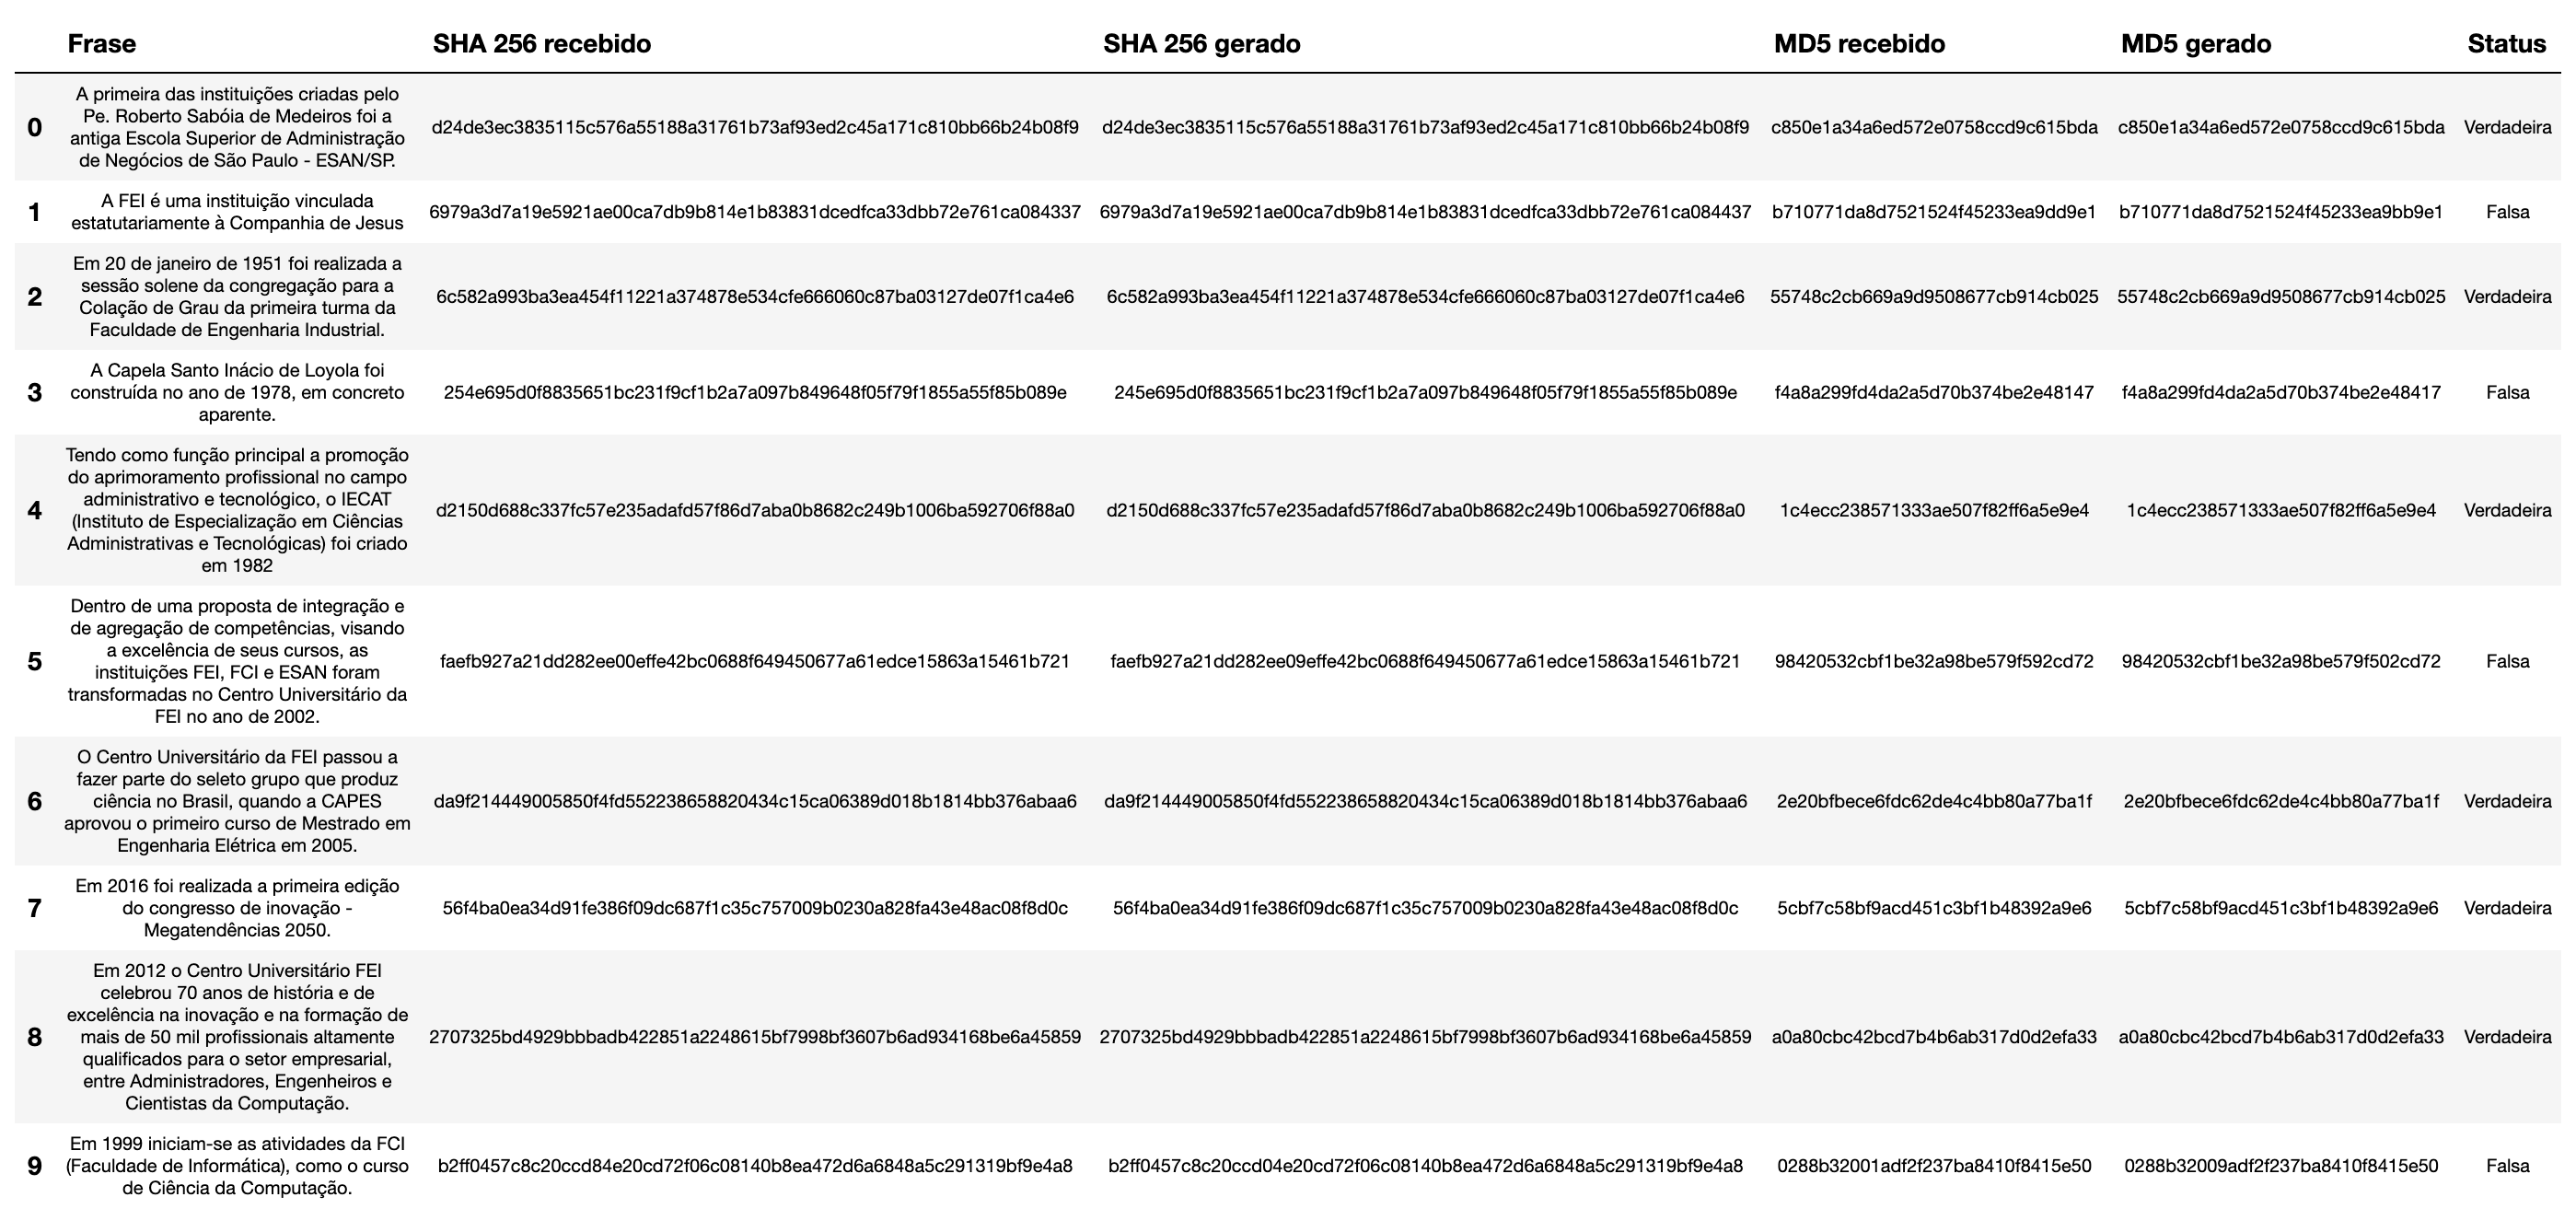
\includegraphics[scale=0.17]{../../tabela.png}
  \caption{Imagem da tabela gerada a partir do código}
  \label{table} 
\end{figure}

\end{document}